\documentclass[leqno,a4paper]{article}
\usepackage{amsmath,amsthm,url,amsfonts,fancyhdr,graphicx,texdraw,amssymb,enumerate}
\newtheorem{proposition}{Proposition}
\newtheorem{theorem}{Theorem}[section]
\newtheorem{lemma}{Lemma}[section]

\mathcode`e=`e

\begin{document}

In what follows, $p$ will be a positive integer prime.

We are considering $\mathcal{A}$, the set of $n$ such that $n-p^2$ is square-free for all $p\leq\sqrt{n}$ and $A(N)$ which counts the elements of $\mathcal{A}$ $\leq N$.

We are perturbed that our naive approach grossly underestimated $A(N)$. The first observation is that we have ruled out those $n\equiv 1\mod\;4$ but we should also rule out $n\equiv 0\mod\;4$ since $4|(n-2^2)$. This actually makes things worse as our naive estimate for $A(2^{23})$ would now be $0.8$ in place of $1.2$ remembering that the actual figure is $9\,384$.

The issue is, I think, that we are assuming that the probability the $n$ is square free, say $P(n)$ to be $1/\zeta(2)$ regardless of the size of $n$. This argument follows from
$$
P(n)=\prod\limits_{p\geq 2}\left(1-\frac{1}{p^2}\right)=\frac{1}{\zeta(2)}.
$$
However, this is not tight unless $n$ is large, for some definition of ``large''. A better estimate is
$$
P_1(n)=\prod\limits_{p=2}^{\sqrt{n}}\left(1-\frac{1}{p^2}\right)=\frac{1}{\zeta(2)\prod\limits_{p>\sqrt{n}}\left(1-\frac{1}{p^2}\right)}.
$$

Now if $n\equiv 2\mod\;4$ or $n\equiv 3\mod\;4$ then $4\nmid(n-p^2)$ so we need to adjust our probability to
$$
P_2(n)=\prod\limits_{p=3}^{\sqrt{n}}\left(1-\frac{1}{p^2}\right)=\frac{4}{3}P_1(n).
$$
Thus the chance of a random $n\not\equiv \{0,1\}\mod\;4$ being in $\mathcal{A}$ is
$$
P_{A}(n)=\prod\limits_{p=2}^{\sqrt{n}}P_2(n-p^2)
$$
and the expectation for $A(N)$ is
$$
\sum\limits_{n=2}^{N/4} P_A(4n+2)+P_A(4n+3).
$$

\begin{lemma}

  $$
  \prod\limits_{p>x}\left(1-\frac{1}{p^2}\right)^{-1}=\exp\left(\sum\limits_{p>x}\sum\limits_{j\geq 1}\frac{1}{jp^{-2j}}\right).
  $$
  \end{lemma}

\subsection{Some computations}

\begin{figure}[tbp]
\centering
\fbox{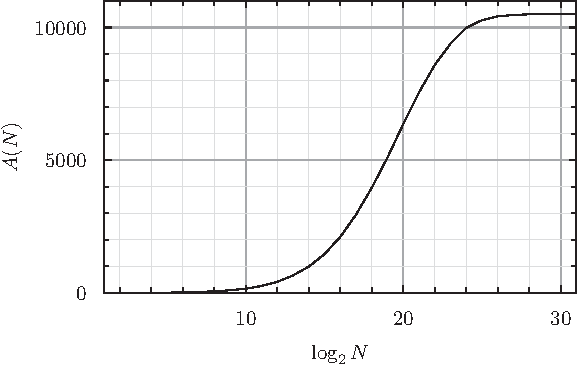
\includegraphics[width=0.9\linewidth] {summary.pdf}}
\caption{Plot of $A(N)$.}
\end{figure}


Running a simple single thread program in Pari even my puny desktop can get to $N=2^{30}$ overnight (actually a little under $10$ hours). Using $4$ threads I went to $2^{31}$. The largest member of $\mathcal{A}$ found was $581\,424\,623$ so by the time we reached $2^{31}$, we hadn't seen one for over $1\,560\,000\,000$ and I conjecture that there aren't any more.



\end{document}
